
\documentclass[index]{subfiles}

\begin{document}
\title{Investigating the efficiency of Cheney stop-and-copy and LISP 2 style mark-compact garbage collection algorithms}
\date{}
\author{}
\maketitle

\section{Research Question}

How does the runtime and collection performance of Cheney's stop-and-copy algorithm compare to the LISP 2 mark-compact algorithm?

\section{Introduction}

Garbage collectors, and the algorithms they use, are incredibly widespread in just about any application one can find in the modern day.

One example of these are higher-level programming languages. Javascript is the sole programming language of the web, and drives the functionality of all webpages. Python is the most popular and rising programming language of today and drives artificial intelligence development. Java, a still very popular programming language encodes \textit{Minecraft}, one of the most popular games of the world, played by millions, and is used in tons of server-side applications worldwide.

The element that these programming languages all have in common is that they are interpreted languages, and they automatically manage memory, by using garbage collectors.

It thus follows that the algorithms behind garbage collection and their relative efficiencies are ever more important to consider, now that more interpreted languages are being run on more and more devices over time. One recent study on this subject has explored the performance differences between different languages running the same program\cite{programming_languages_electricity}, comparing interpreted languages such as Java and Python with manually managed languages such as C++ and Rust. However, the results didn't specifically test garbage collection algorithms specifically, and as each language implements and makes its own tweaks to its own unique garbage collection algorithm, it's hard to say if one base garbage collection algorithm is better than the other using these results alone.

Other contemporary research on the subject has become increasingly complex, factoring in new algorithms or combining old algorithms, however, many assume the basic algorithms as known information, and haven't tested simple algorithms on modern hardware. This paper aims to shed light on the essential component of higher level languages that many programmers tend to look over, presenting information in an easily digestible way, as well as applying that knowledge practically by implementing a simple stop-and-copy and mark-compact garbage collection algorithm in the same programming language in an abstracted way, and comparing the performance of the two in this controlled environment.

\subsection{Methodology}

To fully compare and contrast the differences between these two algorithms, as well as to make educated analysis of the results later, a basic understanding of how memory works in a program, the basic terminology concerning memory management, and what garbage is needs to be researched and understood.

Then research will be done on the basic steps in each algorithm: including when garbage collection is run, how live objects are determined, and what objects are moved where during the compaction process of each algorithm. This will be accompanied by code snippets of how the algorithms are implemented in this paper in the Rust programming language.

Next, the collection performance of each algorithm (how long it takes to clean up the garbage) as well as the runtime performance of each algorithm, (such as accessing the data structure and its values during a traversal of the memory) will be tested and the results recorded.

Finally, research will be done on the basics of hardware caches and organization of memory in modern systems, as one algorithm or another due to its compaction process could support a faster runtime of the program after collection of garbage, and this information will be used to critically analyze the results of the performance of the two algorithms.

\section{Background}

The data of all computer programs are stored in a place we call memory. Whenever one wants to make room for new data, one must allocate memory to free space. And whenever one wants to remove data, one must deallocate that memory, back into free space.

In modern computers, there are two places where the program can allocate memory: the stack and the heap\cite{the_rust_programming_language}.

In the stack, whenever one wishes to allocate something, all one has to do is bump a pointer's memory address up to determine where our next boundary of free memory is\cite[Chapter~4.1~What~is~Ownership?]{the_rust_programming_language}. However, whenever one wishes to deallocate memory, they must do so from top to the bottom. Thus, the stack always consists of a block of contiguous used memory, and a block of contiguous free memory.

\begin{minted}[breaklines]{rust}
    free = 4
    memory = [data1, data2, data3, NULL, NULL, NULL]
\end{minted}

However, most of the memory of programs aren't allocated linearly and deallocated in the exact opposite order. Thus, garbage collection is most concerned with the heap, because this is is where objects can be accessed at random, and where objects with dynamic sizes (that is, that is, sizes unknown at the time we compile our program) can be stored.

However, in a running program, when there are dynamicly sized objects expanding and decreasing in size, objects that are allocated but no longer in use, there needs to be a way to reclaim this memory automatically. Thus memory management aims to determine which parts of the heap are ``free'' memory, and which sections are ``used'' memory.

\subsection{Memory Management Techniques}

There are several ways to manage memory in a language. One is by manually allocating and deallocating: the programmer specifies exactly how much memory is needed at a specific time, and decides when something should be deallocated. In lower-level languages, this is normal. However, manual allocation often requires a lot of experience to learn, and even with it, requires much more time to think about and write a program. It could also easily result in many types of bugs, such as using memory that is already freed, freeing memory twice, and not freeing memory in the first place \cites{garbage_collection_overview_uw}[Chapter~1]{gc_handbook}

Hence, to alleviate the burden of having to keep track of manual memory management, many modern programming languages use automatic memory management. There are many different ways to automatically manage memory. The only types of garbage collectors this paper is concerned with are tracing garbage collectors, which, as their name suggests, directly check objects to determine if they are ``alive'' (used by the program) or ``dead'' (not in use any longer)\cite{a_unified_theory_of_garbage_collection}. This is usually determined by traversing some kind of tree of the live objects\cite[Chapter~1]{gc_handbook}, then declaring everything else garbage.

The main concept of garbage collection algorithms consists of just two steps: to create a new object, \verb+allocate()+is called, which calculates if there is enough free space on the heap and occupies that section of memory. But if the heap is full, or if the programmer wishes to optimize the heap at any time, then the \verb+collect()+\cite{gc_handbook} function is called, to find all the garbage and move them in the case of copying and compacting collectionrs. These two functions of the two different garbage collection algorithms will be discussed in depth in the following sections.

\subsection{LISP-2 Sliding Mark-Compact Algorithm}

One easy implementation of the mark-compact garbage collector is the \textit{sliding} LISP 2 mark-compact garbage collection algorithm.

\begin{figure}[H]
    \centering
    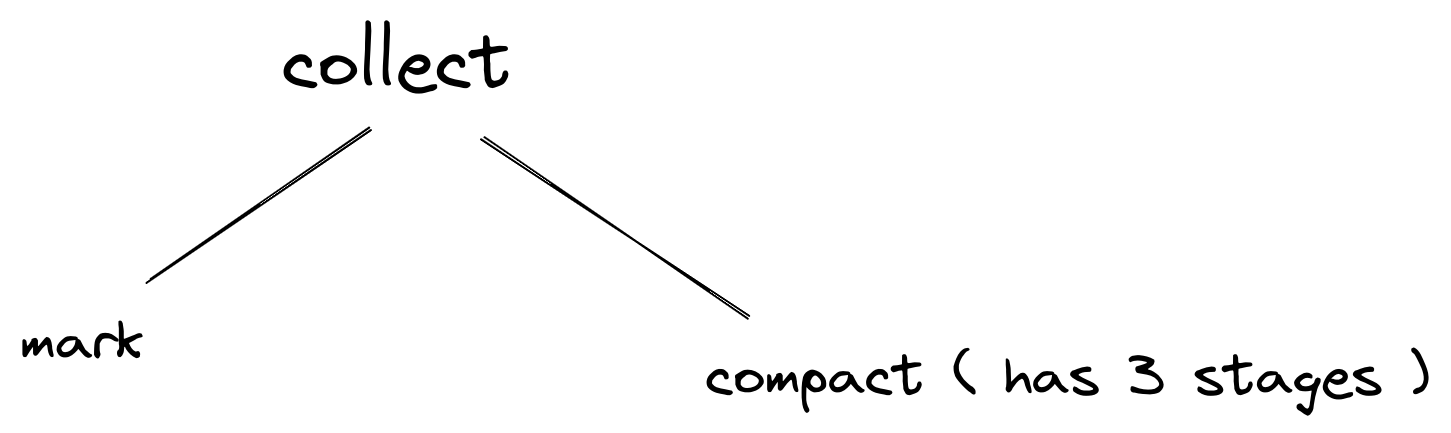
\includegraphics[scale=0.3]{pics/mark-compact-overview.png}
    \caption{Basic overview of mark-compact algorithm}
\end{figure}

The \verb+collect()+ function of this mark-compact algorithm can be broken down into two stages: the \verb+mark()+ stage, where we find out which objects are ``living'' and the \verb+compact()+ stage, where we perform a series of computations to ``slide'' the living objects down into one end, compacting the heap in the process and freeing up space\cite[Chapter~3]{gc_handbook}.

\subsubsection{The Marking Stage}

To determine which objects are alive and dead, we first attempt to traverse the entire heap through the graph of objects. We start from the root nodes, located on the stack\cites[Ch~3~Marking]{redhat_openjdk}[Chapter~3]{gc_handbook}, adding the objects that they reference to a worklist (which can either be a stack or a queue, to traverse breadth-first or depth-first). Then for every object in the worklist, we mark the object if we haven't already, then add their children to the worklist. This action is iterated over and over again, and so on, until the worklist is exhausted. Accessible objects are objects that can eventually be reached by this recursion of reference from the roots. Objects that are then found to be inaccessible (because they are unmarked) are defined as `garbage' and can be ignored in the \verb+compact+ phase.\footnote{See Appendix A for the code for the marking stage}

There are several ways to ``mark'' an object that is accessible\cite[Chapter~3]{gc_handbook}. One simple way is to mutate a specific, dedicated boolean field of the object. This could be the same field as used for the forwarding address necessary for the compact stage as discussed later\cite[Chapter~1]{gc_handbook}.\footnote{This implementation method is what the program chose, but another method with difference performance implications is the use a bitmap (an array of bits, basically) where each index corresponds to each object in the heap, which is marked 1 or 0 to show that it is alive (1) or dead (0)\cite[Chapter~3]{gc_handbook}}

\subsubsection{Compact Stage}

The compaction stage of the mark-compact algorithm can be broken down into three parts, and in each part, the heap is traversed in its entirety.

The first stage is to calculate the location of where the living object will slide down after copying. We do this by initializing a \verb+free+ pointer starting at the very bottom of the heap. Then we iterate over all the memory in the heap. For every object that we marked (which we determined by checking the \verb+forwarding_address+ field of each object we mutated), we set the new address of the object in question to the free pointer, then bump the free poitner by the object's size \cites[Chapter~3]{gc_handbook}[Sections~3.3--3.5]{redhat_openjdk}.\footnote{See Appendix B for code for calculating the forwarding address of marked objects}

The second stage of garbage collection is to update the references of each marked living object to point to the new \verb+forwarding_address+ of where they'll eventually be moved. We do this by iterating over the heap a 2nd time, only looking at marked objects again. Then for each reference (or it could be thought of as each ``child'' object that a ``parent'' object references), we retrive the \verb+forwarding_address+ for that referenced object and set that as the new reference to the object \cites[Chapter 3]{gc_handbook}[Sec.~3.4]{redhat_openjdk}.\footnote{See Appendix C for code that updates the references of each object}

\begin{figure}[H]
    \centering
    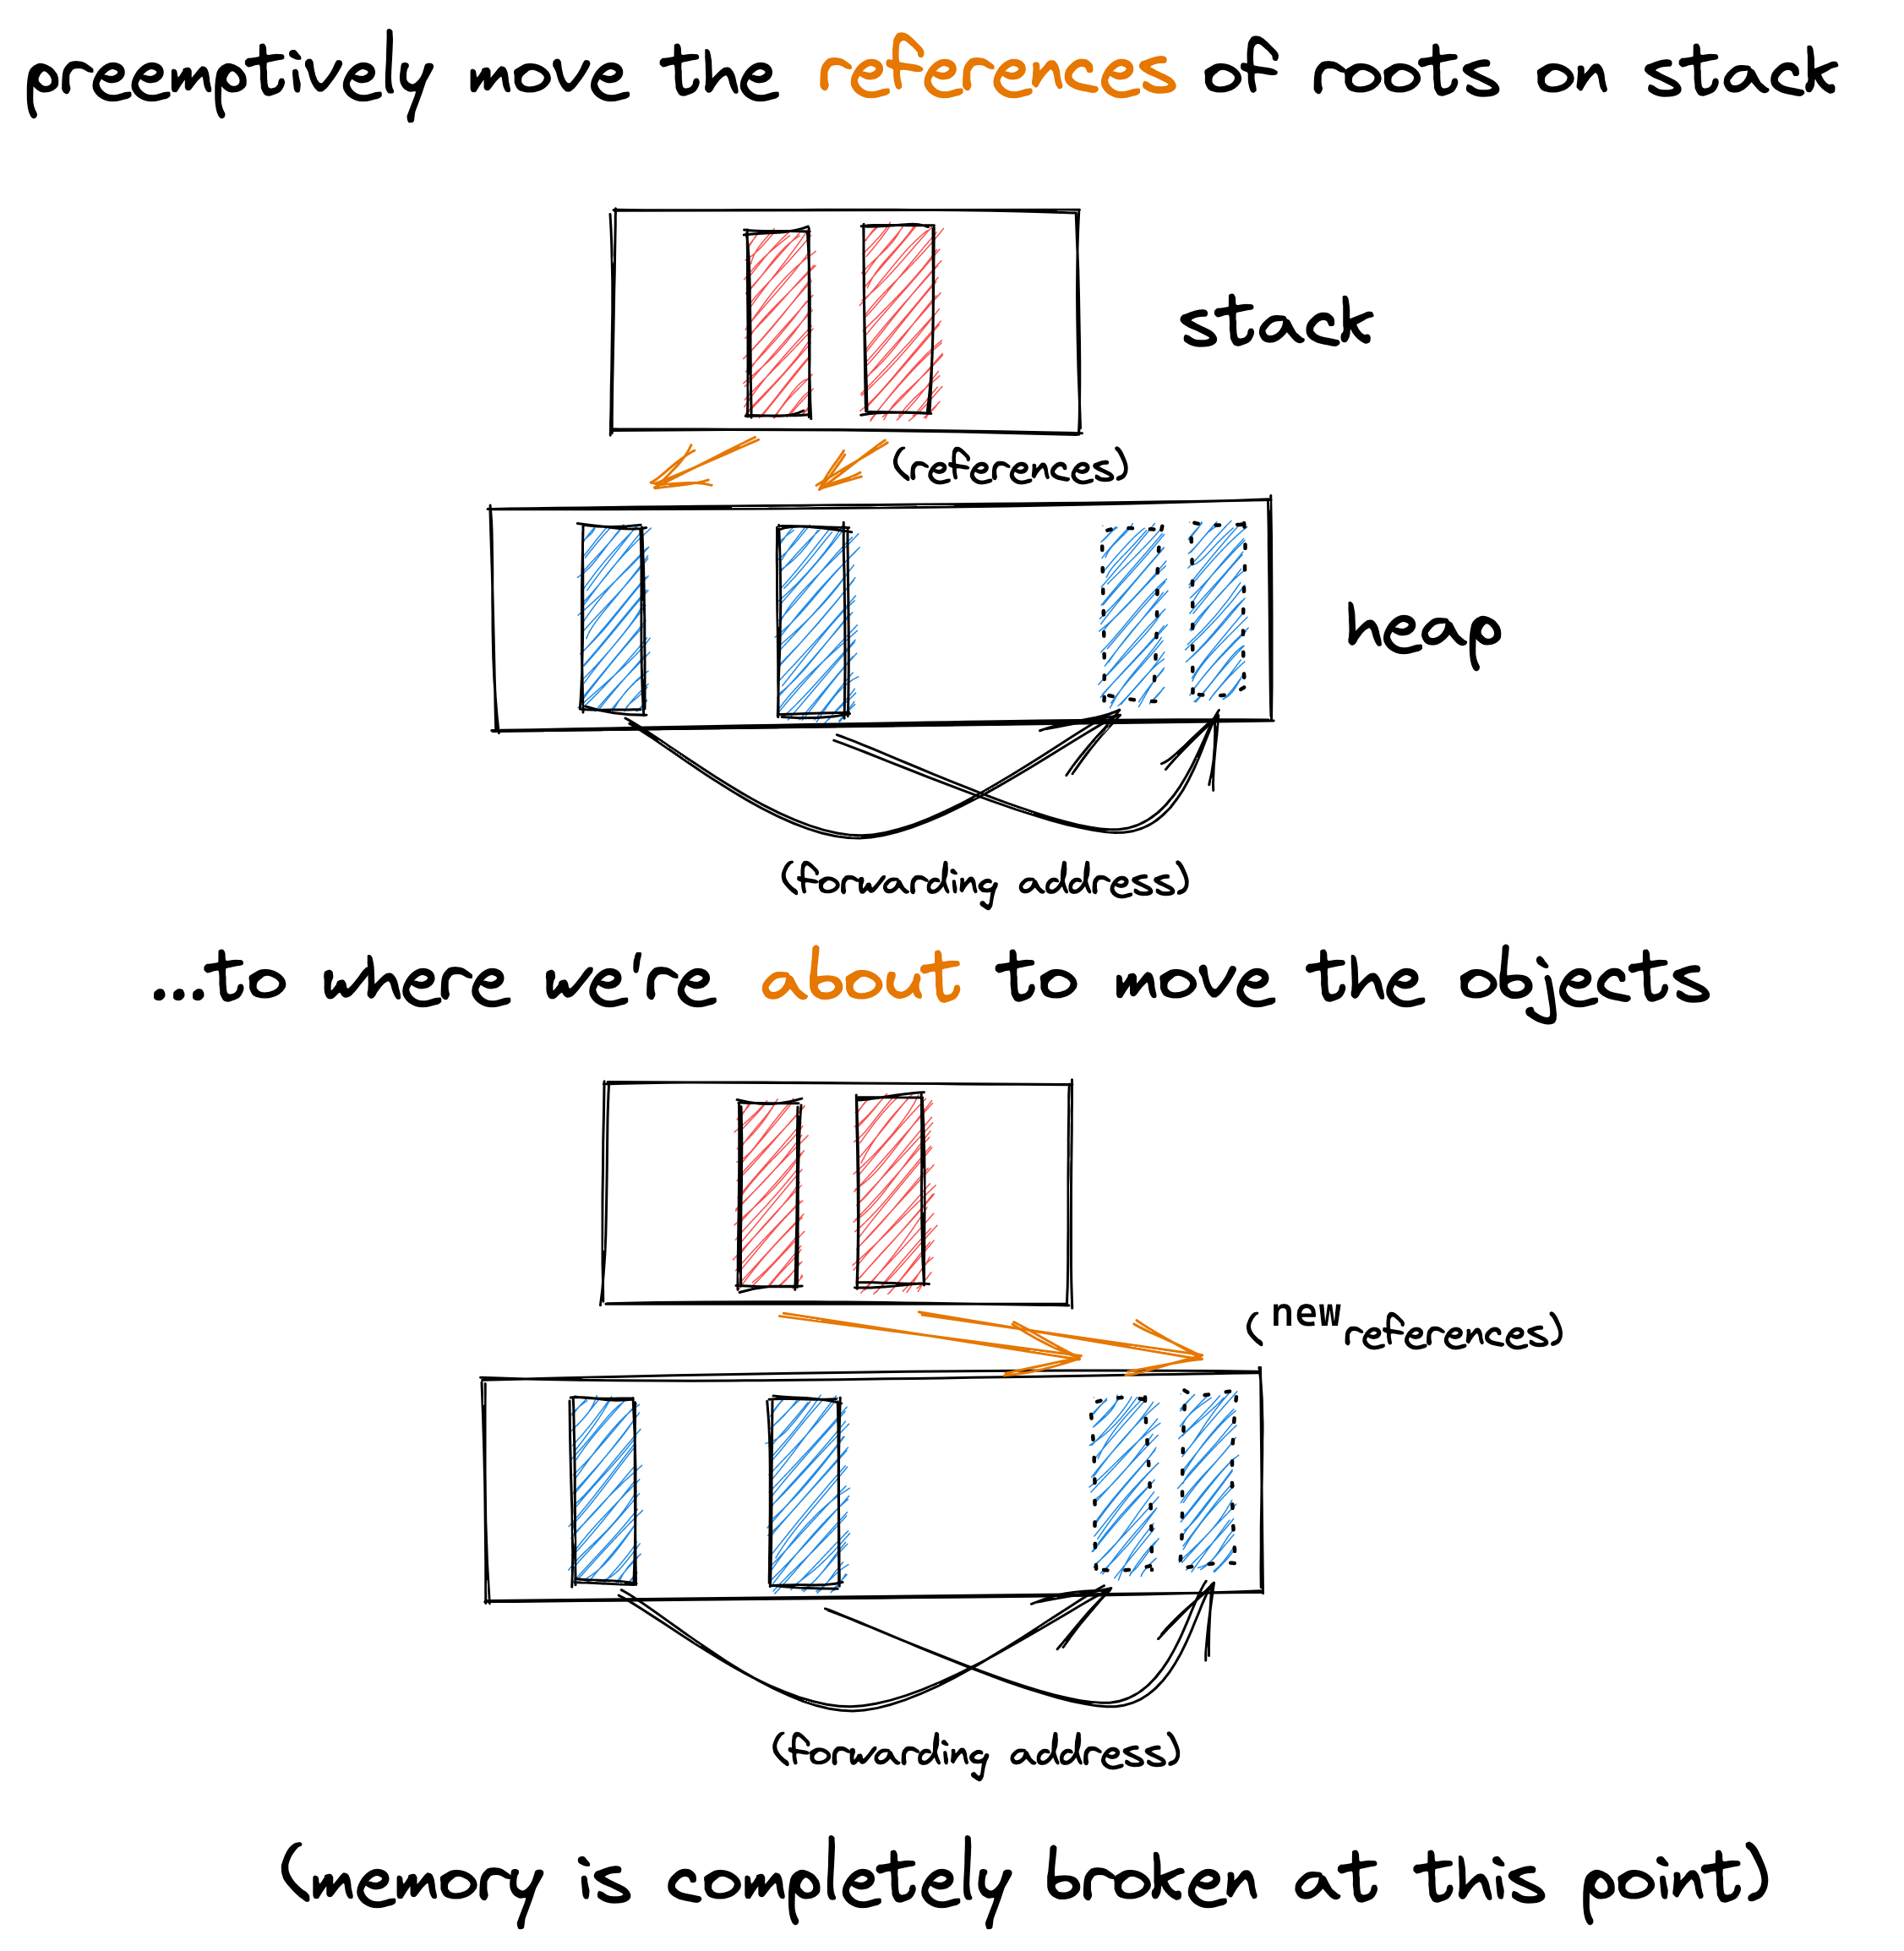
\includegraphics[scale=0.3]{pics/update-references.png}
    \caption{Updating references in the compact step of mark compact, visualized.}
\end{figure}

Finally, we can actually move the objects over to where their \verb+forwarding_address+ points to

\begin{figure}[H]
    \centering
    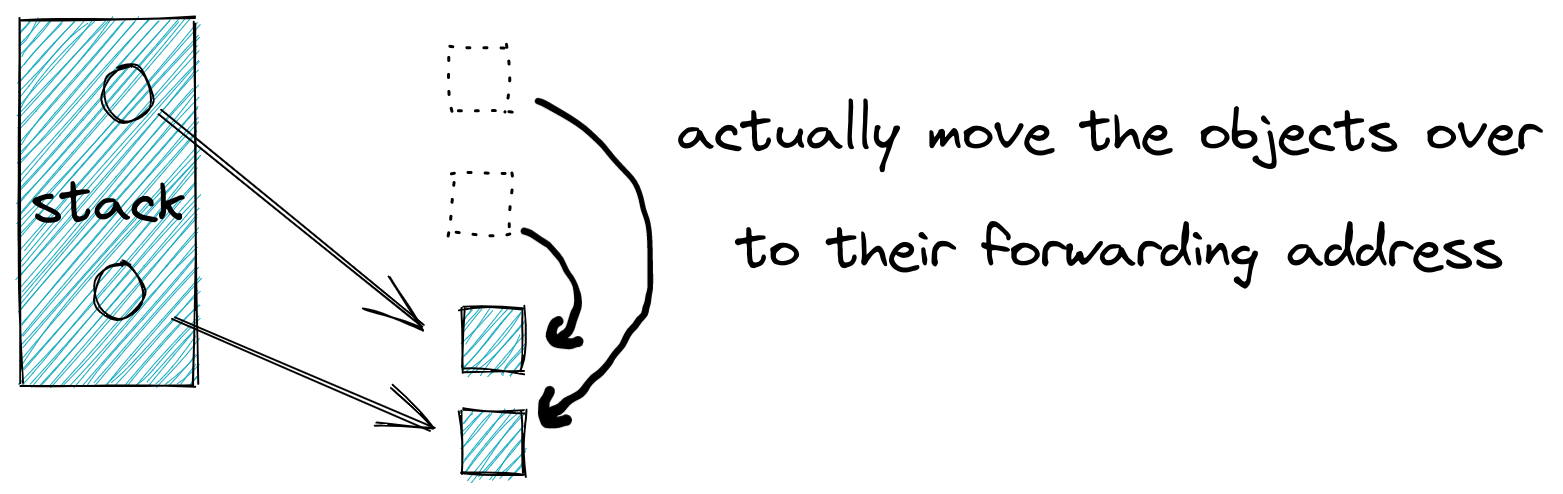
\includegraphics[scale=0.25]{pics/actually-move.png}
    \caption{Actually moving objects, the ``compact step'' in the compact step of mark compact, visualized.}
\end{figure}

We do this by traversing the marked objects in the heap a 3rd time, then making \mintinline{rust}{std::mem::swap} calls between where the object is currently located and their \verb+forwarding-address+. It's important to note here, that the sliding mark-compaction algorithm \textit{maintains the order} of which the objects were on in the original heap, as well as moves objects \textit{more closely together} towards the beginning end of memory, which is why the LISP 2 algorithm is known as a ``sliding'' implementation of the mark-compact algorithm.\footnote{See Appendix D for ``sliding'' code}

The order of compacted objects is an important destinction to make in the comparison between the mark-compact and stop-copy garbage collection algorithms, because Cheney's stop-copy collection algorithm does not preserve the order of objects in memory.

\subsection{Cheney's Stop-and-Copy Algorithm}

The second type of garbage collector investigated in this paper is Cheney's stop-and-copy algorithm, which uses double the memory of the LISP 2 mark-compact algorithm, but in return, is able to mark and copy objects all in one pass of just the live objects.

When initializing the heap using this algorithm, the beginning contiguous heap is split into two sections, named a \verb+from_space+ and a \verb+to_space+\cite[Chapter~2]{gc_handbook}.

\begin{figure}[H]
    \centering
    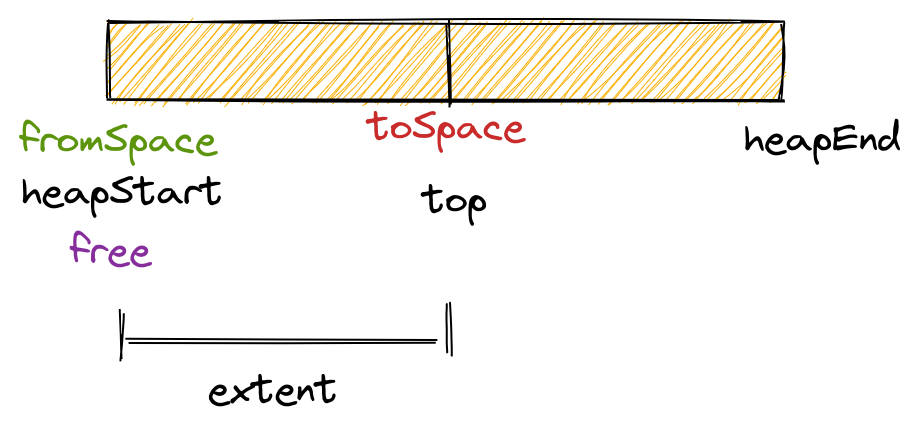
\includegraphics[scale=0.3]{pics/split-heap-diagram.png}
    \caption{Picture of what the heap looks like for a stop-and-copy algorithm}
\end{figure}

Like the mark-compact algorithm, on every allocation, it checks if the heap has enough free space by attempting to bump the \verb+free+ pointer and check if it's less than the \verb+top+ of the heap.\footnote{See Appendix E for allocation code}

\begin{figure}[H]
    \centering
    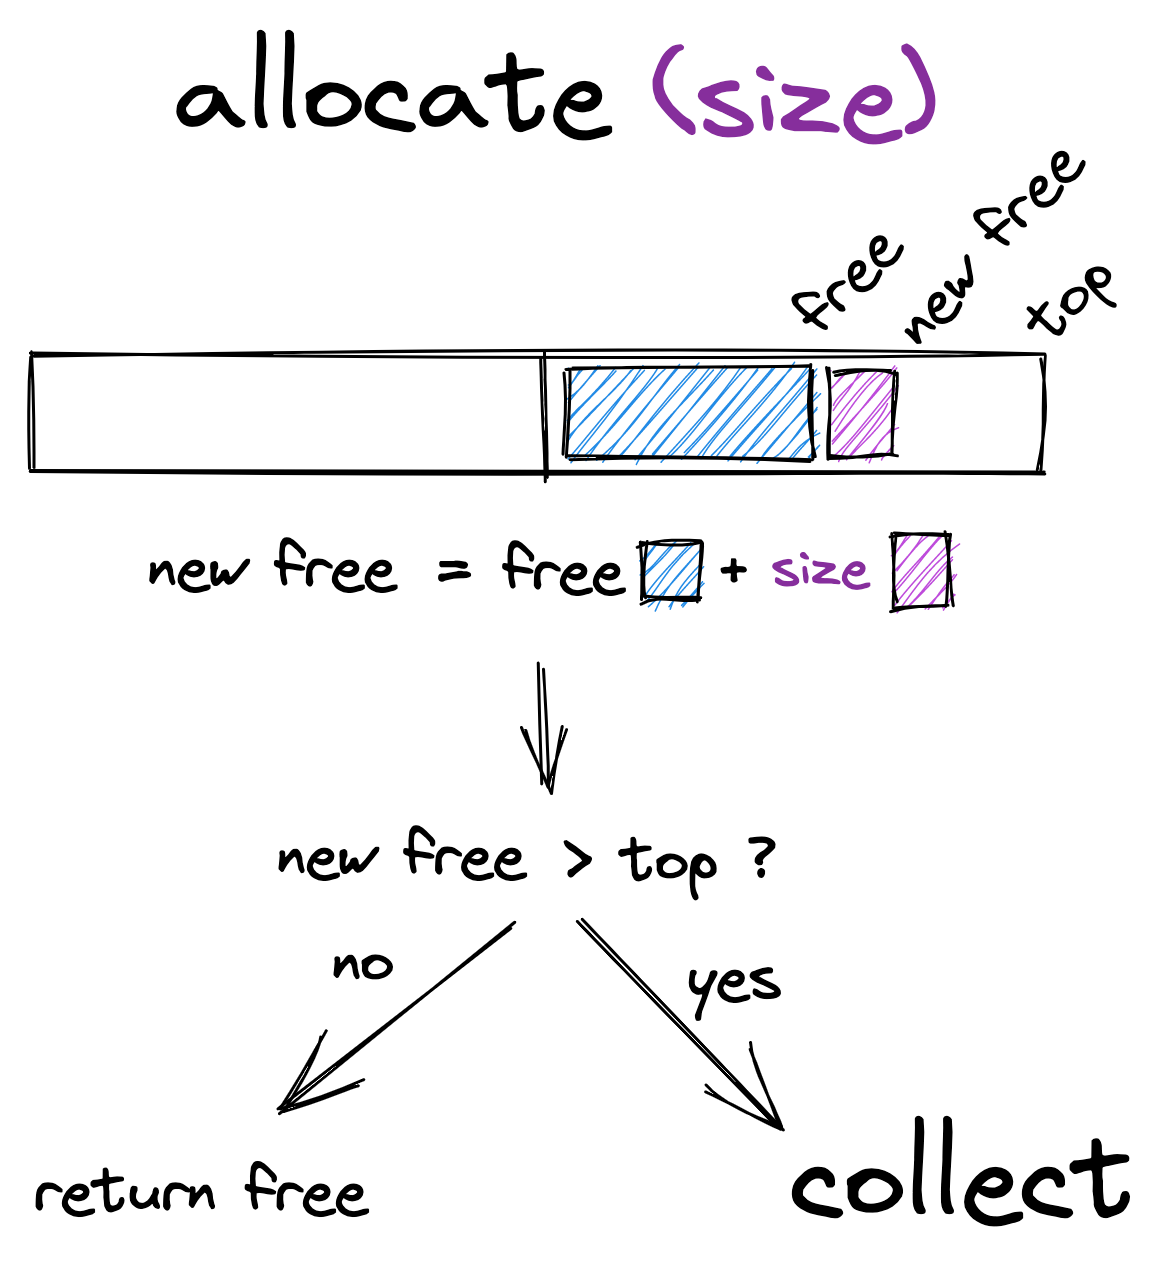
\includegraphics[scale=0.3]{pics/allocation.png}
    \caption{What checking for allocations looks like.}
\end{figure}

In this case, because the heap is split in half, we check that the \verb+free+ is not greater than the end of the heap but rather that it is not greater than half of the size of the heap. Once the heap does end up filling up, we can no longer allocate a new object on the heap and thus must call the \verb+collect()+ function of the stop-and-copy garbage collection algorithm.

\subsubsection{Cheney's Algorithm}

Right as the \verb+collect()+ function is called, we flip the \verb+from_space+ with \verb+to_space+.\footnote{See Appendix F for swap code}

\begin{figure}[H]
    \centering
    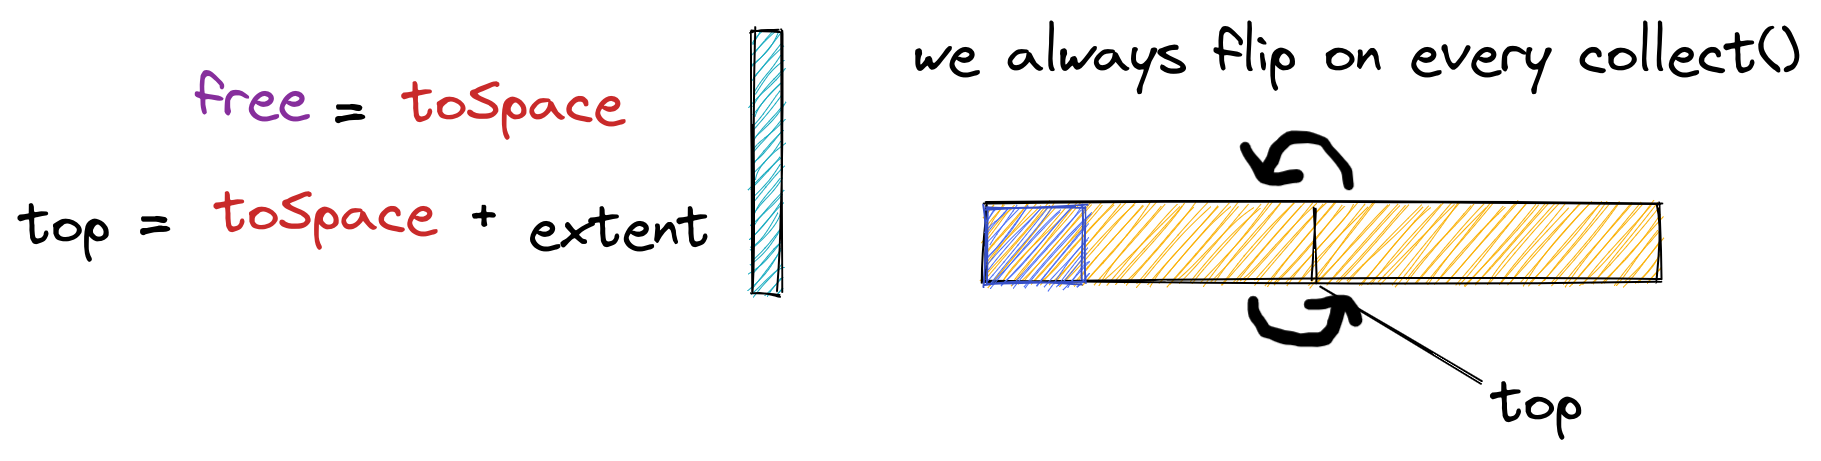
\includegraphics[scale=0.25]{pics/flipping.png}
    \caption{flipping}
\end{figure}

Then we follow that by \verb+copy+ing the initial children of the roots reachable by the program into \verb+to_space+. Note that the references that these children newly copied to \verb+to_space+ hold still point to objects in \verb+from_space+\footnote{See Appendix G for initial population population of worklist code}

Inside the \verb+copy+ function, we move the children of the roots over (if they haven't been moved already), then we update the \verb+forwarding-address+ of their old location on \verb+from-space+ to point to their new location on \verb+to_space+.\footnote{See Appendix H for copy code}

\begin{figure}[H]
    \centering
    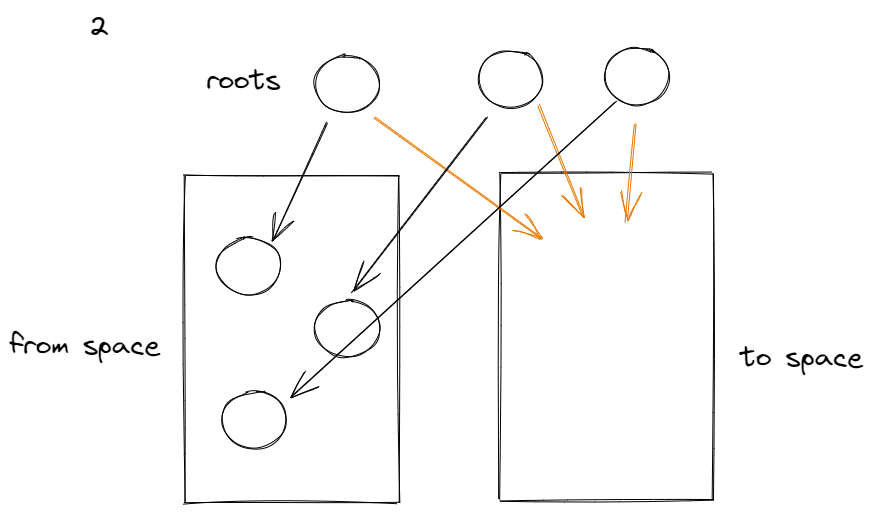
\includegraphics[scale=0.3]{pics/visualization-of-worklist.png}
    \caption{The algorithm for stop and compact. During the collect function, objects in from space are copied to to space, and their forwarding addresses are updated to point to the copied objects in to space.}
\end{figure}

Now, the objects, and references of objects in \verb+to_space+ effectively act as a worklist. We repeatedly iterate over the objects in \verb+to_space+, until we reach the end of all the objects in \verb+to_space+. For every object that we then encounter (including the roots that we just moved), we find their references, move them over to \verb+to_space+ if we haven't already, and then update the references to point to \verb+to_space+. (If their references have already been moved, then we can just use their \verb+forwarding_address+ that we updated on the \verb+from_space+ to point to the right location)\footnote{See Appendix G for code that copys remaining objects}.

It should be noted that because the objects in \verb+to_space+ act as a worklist, stop-copy is breadth-first by default and this cannot be changed, as opposed to mark-compact, which can choose between using a stack and queue (and therefore between breadth-first or depth-first) in the marking stage.

Upon reaching the end of the \verb+to_space+, garbage collection is done, because all live objects have been copied to the the effective heap. At this point, the \verb+from_space+ is basically ignored, and the \verb+to_space+ becomes the effective heap, until the next cycle of garbage collection occurs.

\section{Experiment}

From the algorithms above, one can infer that for a garbage collector, or more specifically, compacting collectors, there are two areas where pure performance can be measured\footnote{Because objects are compacted in both, allocations are fast. This is not the case for mark-sweep, where the performance of the mutator is potentially much worse}. This is during the \verb+collect()+ part of the algorithm, when the graph of live objects is being traversed and objects are being moved to their compacted points, as well as the runtime performance of the program, when the objects on the heap are being accessed after garbage collection.

\subsection{Method}

To test and compare these two algorithms, both were implemented as part of a library for the Rust programming language, a low-level programming language with comparable performance to C with its own novel model of memory management. Being implemented in a low-level programming language, the performance of the algorithms would not be subject to performance impacts of that language's garbage collector.\footnote{Snippets source code for the algorithms can be found in the Appendix, as they have been referenced throughout the paper. The full source code can be found at \href{https://github.com/SpicyRicecaker/gc-representation-rs}{https://github.com/SpicyRicecaker/gc-representation-rs}}

To generate the testing data, a binary tree will be created with an arbitrary size of \(1,000,000\) objects.

Each node will be generated linearly via appending to a vector, with the pointer to nodes on that vector abstracted as indices into that vector. Each parent node will have two child nodes, and they'll be added via \textit{breadth-first} recursion. This means that a full layer is filled with nodes in the tree before moving onto the next layer, so all layers will be filled except the layers containing the leaf nodes.

Next, to make the data structure slightly more dynamic than a binary tree and more representative of real objects in a program, parents are then linked randomly to children using a seeded random generator. A seeded number will allow for generated values to be consistent across algorithms and across multiple trials, making test results more consistent and much more reproducible.

Nodes are then removed randomly from the tree (at an arbitrary number of layers under the root, such that the entire tree won't be deleted). At this step, the number of nodes deleted is \textbf{varied}, and a calculated ratio of dead to live objects recorded after garbage collection serves as the independent variable for the graphs below. This variation will allow tests for different scenarios of what a full heap might look like in a real program: made of many live, or many dead objects that need to be collected.

Finally, to measure the collection performance, for each heap of each of the two algorithms, \verb+collect()+ is run, and the time taken measured and recorded (via benchmark program discussed later).

To measure the runtime performance, the heap that each respective algorithm has just operated on will be traversed, the value of all nodes in the graph summed up. There will be two traversals: one using breadth-first search, and one using depth-first search. The time taken to completed these traversals will be recorded.

The testing framework used in this experiment will be the \verb+criterion+ crate in Rust. This crate automatically runs each function for a set amount of time in the beginning to prep the cache\cite{brookheislerAnalysisProcessCriterion}, which is especially relevant for garbage collection, as the way objects are arranged in memory will be different after garbage collection is run, which would affect the layout of objects in the cache. It also runs each test multiple times in order to reach a target runtime length, which increases the certainty in the average value that it returns for the time it took to complete the function\cite{brookheislerAnalysisProcessCriterion}.

\subsection{Data}

\begin{figure}[H]
    \centering
    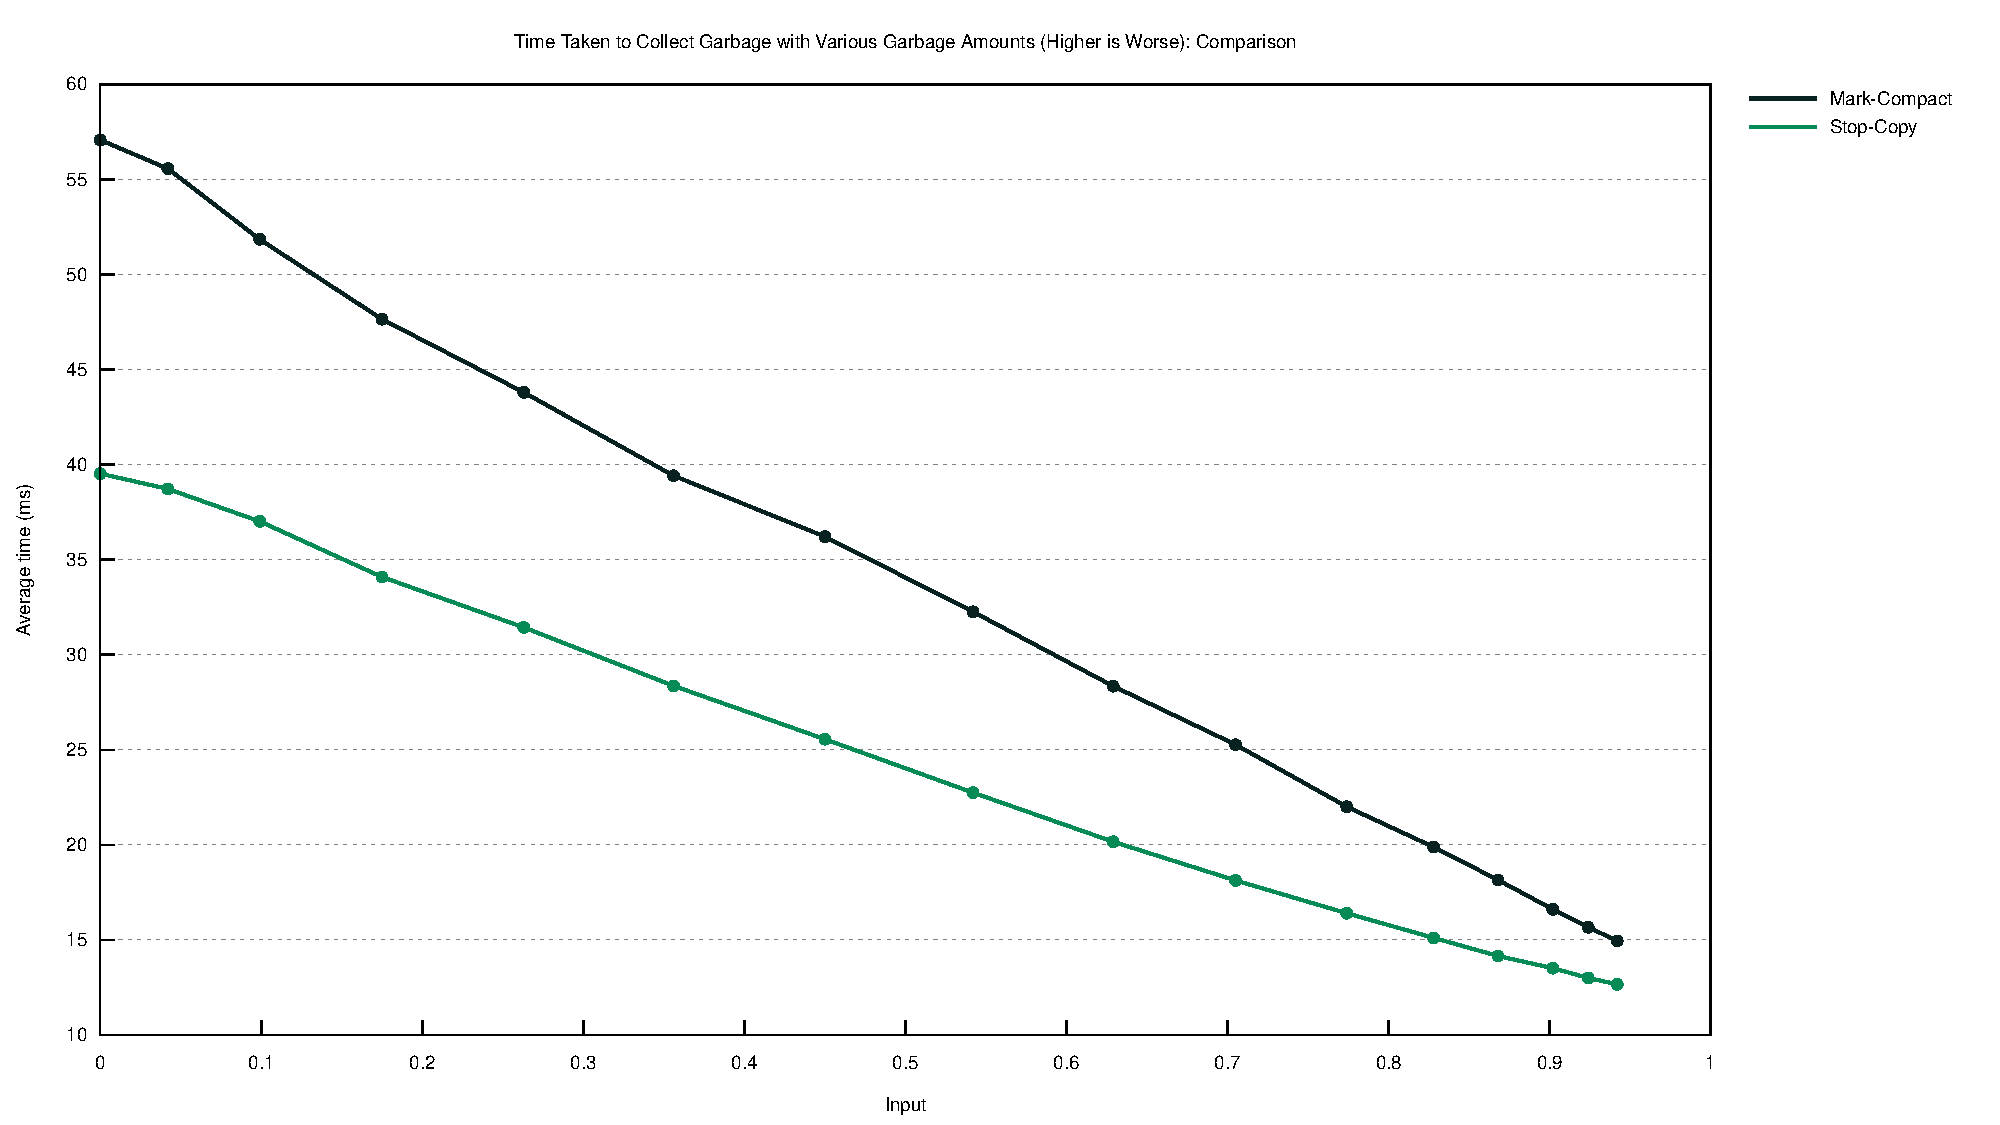
\includegraphics[width=0.9\textwidth]{pics/collect.pdf}
    \caption{Collection performance: Time Taken to Collect garbage with Various Garbage Amounts, where the \(x\)-axis demonstrates the ratio of dead to live objects in the heap before removal.}
\end{figure}
\begin{figure}[H]
    \centering
    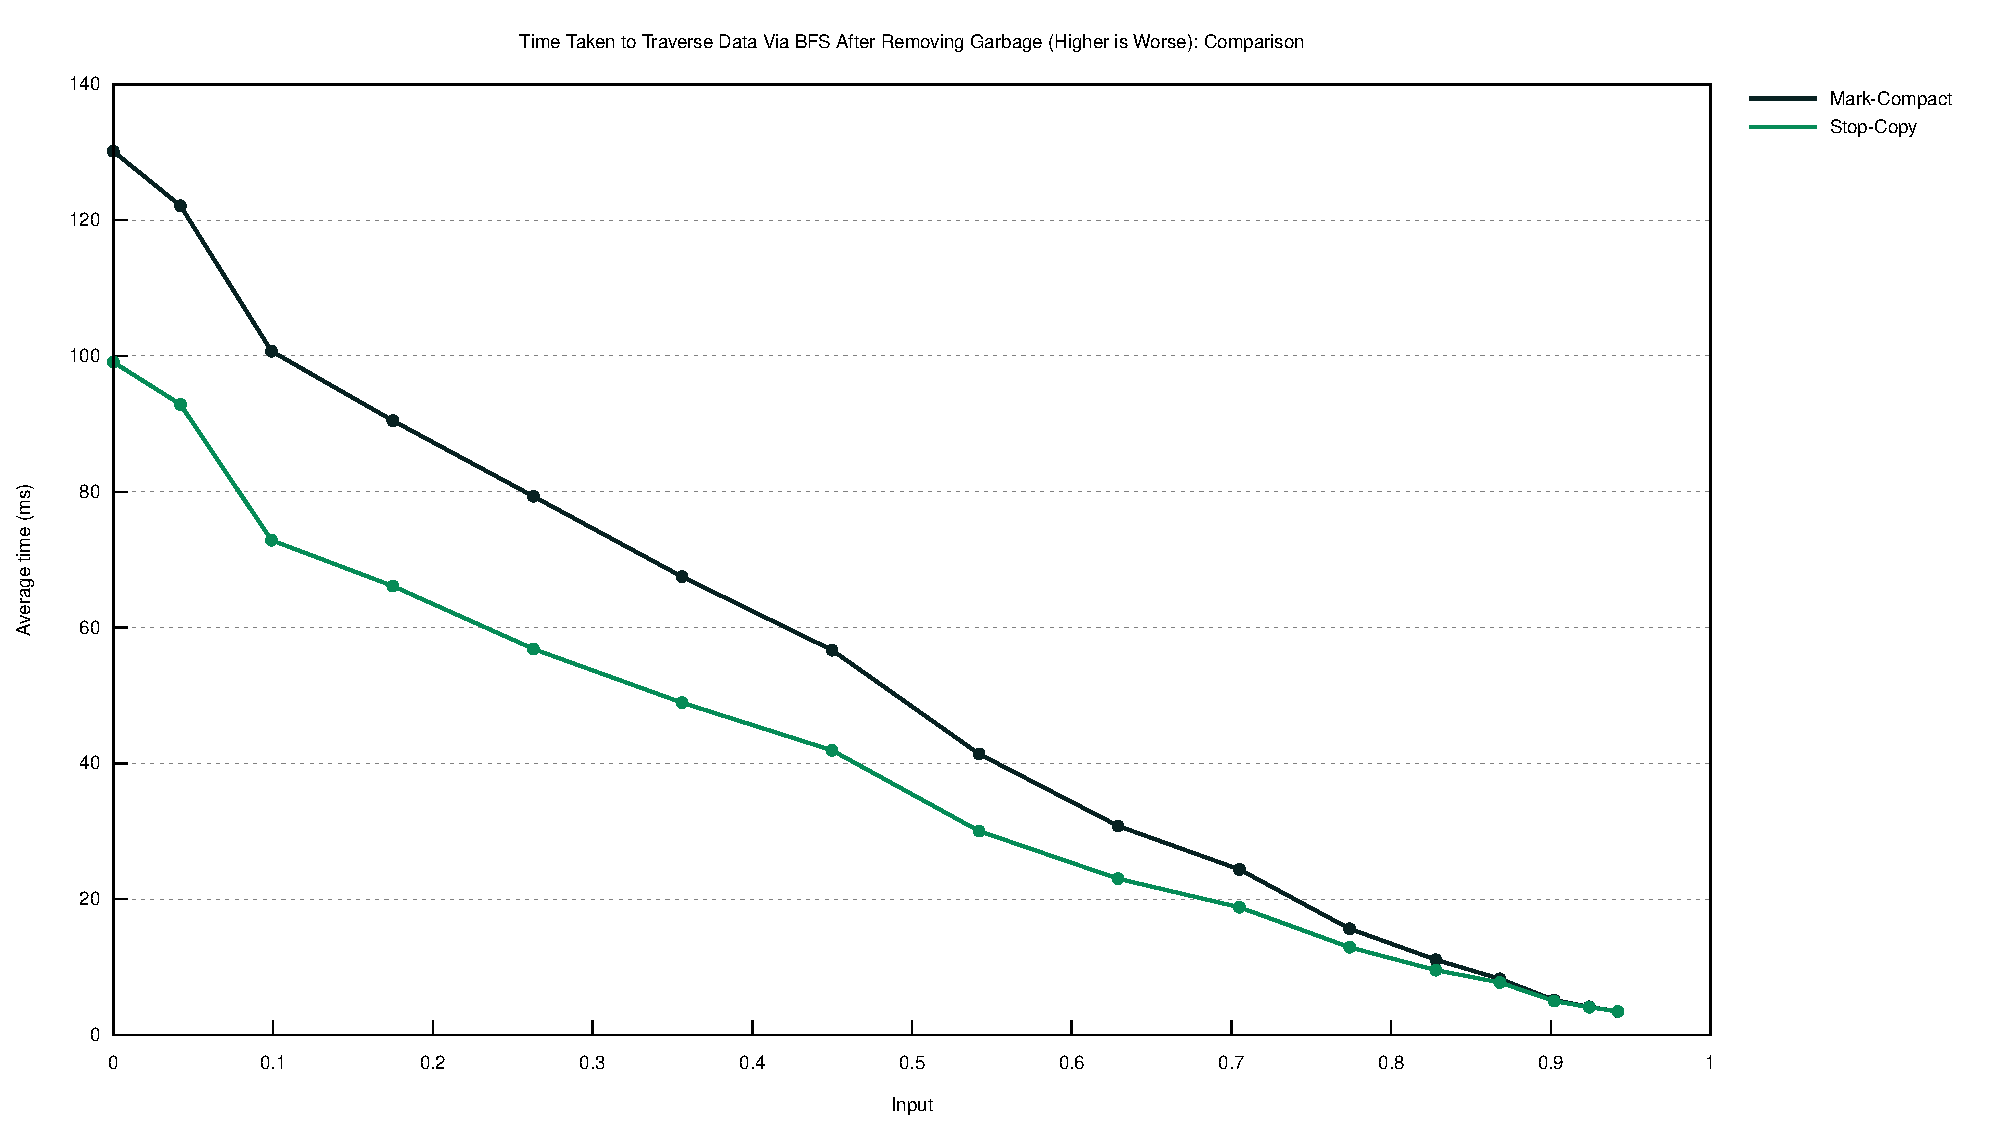
\includegraphics[width=0.9\textwidth]{pics/bfs.pdf}
    \caption{Runtime Performance: Time Taken to Traverse Data Via BFS after removing Garbage, where the \(x\)-axis demonstrates the ratio of dead to live objects in the heap before removal.}
\end{figure}
\begin{figure}[H]
    \centering
    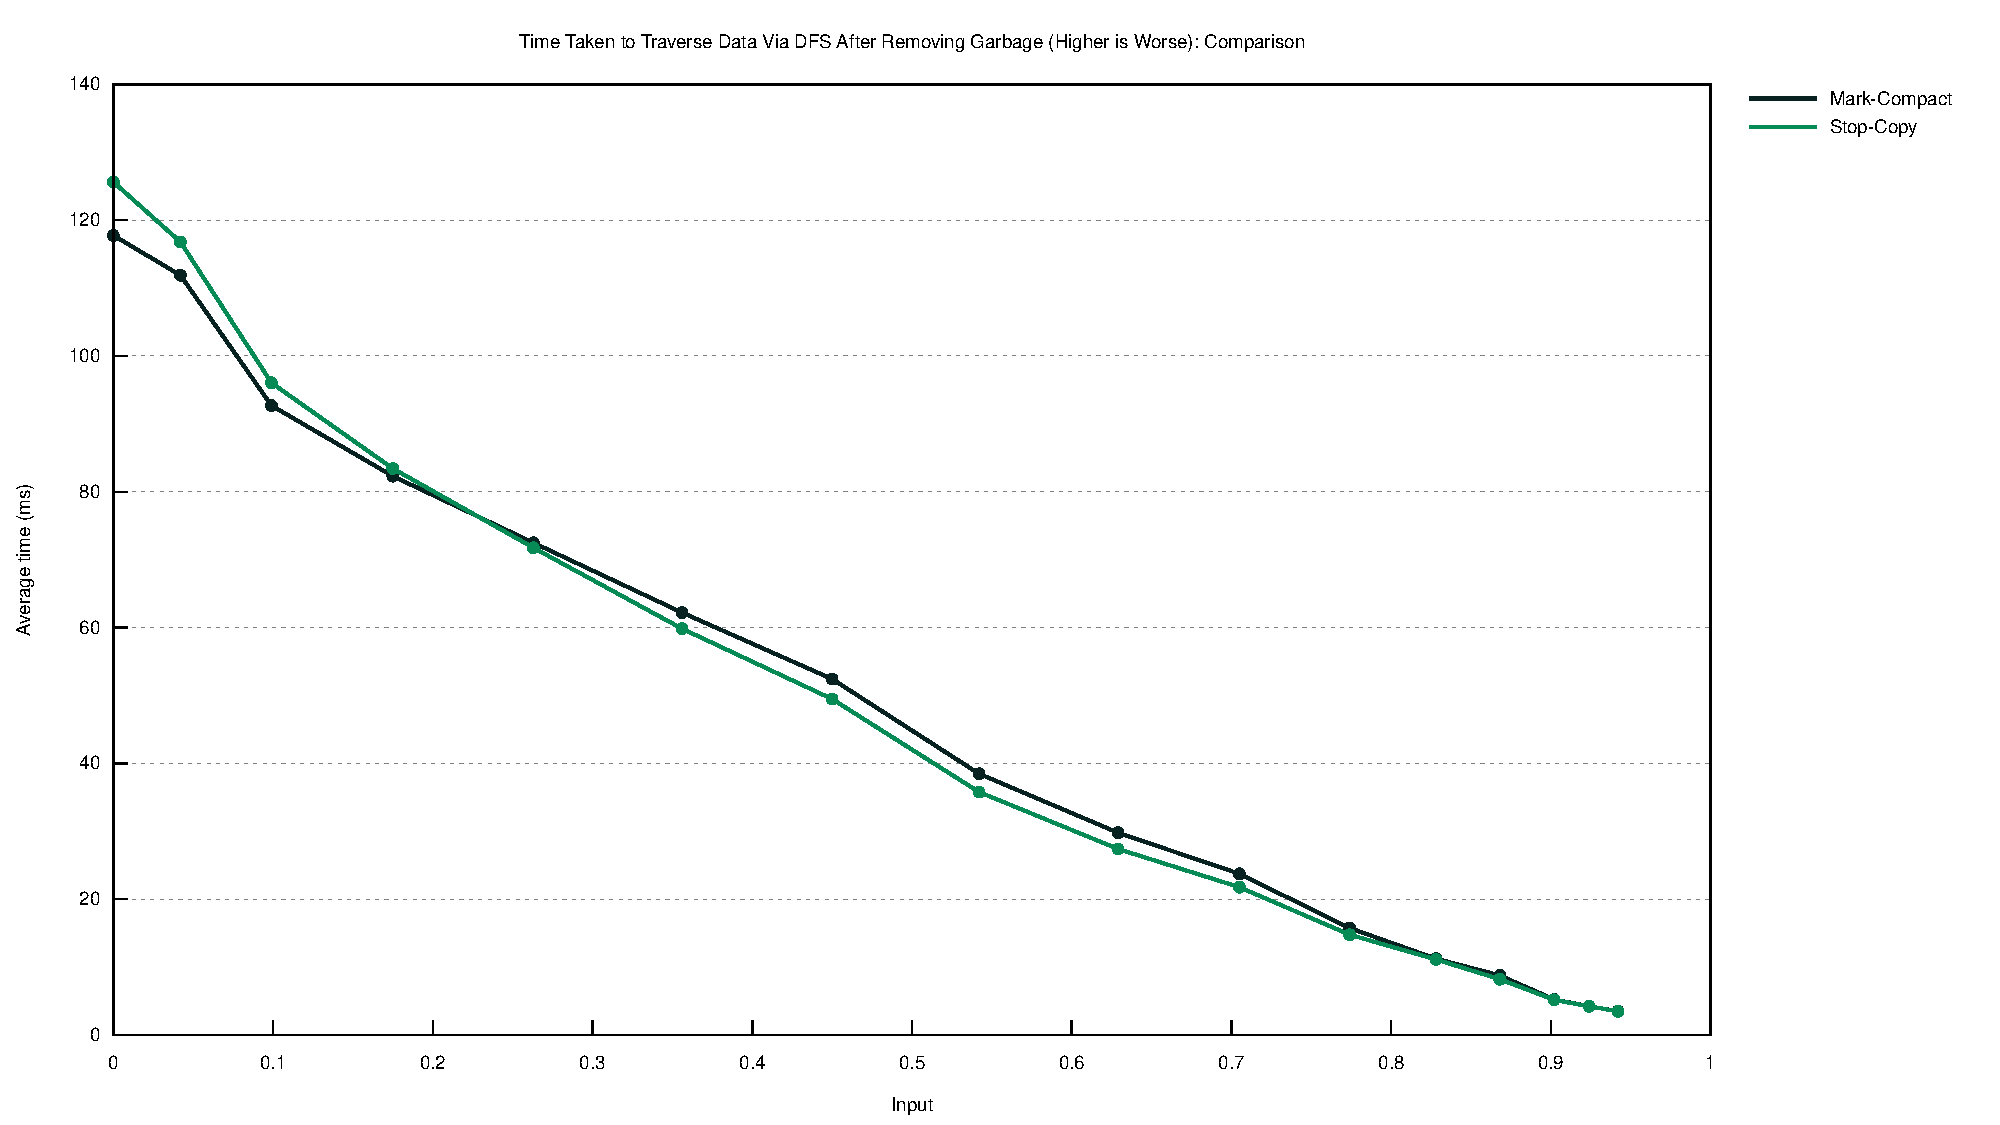
\includegraphics[width=0.9\textwidth]{pics/dfs.pdf}
    \caption{Runtime Performance: Time Taken to Traverse Data Via DFS after removing Garbage, where the \(x\)-axis demonstrates the ratio of dead to live objects in the heap before removal.}
\end{figure}

\subsection{Observations and Analysis}

\subsubsection{Collection Performance}

Initially, with no garbage in a collection cycle, the collection performance of Cheney's algorithm is already as fast as around \(1.4x\) the speed of the LISP 2 algorithm. This makes sense because the mark-compact algorithm had to traverse the heap 3 times, whereas Cheney's only had to traverse through the heap once to determine the live and dead objects. However, Cheney's algorithm is not \(3x\) as fast as the LISP 2 style algorithm. This is perhaps because of the fact that Cheney's algorithm had to copy every single live object in the entire heap (as there were no dead objects) from \verb+from_space+ to \verb+to_space+ regardless of its current position, whereas the mark-sweep algorithm \textit{did not have to move any objects at all} because objects were already in their compacted places for mark-sweep. Intuitively, copying memory around is fairly expensive.

Overtime, however, it seems that the collection time of both algorithms trend down linearly, with the mark-compact collection algorithm having a consistently higher value in each iteration. This also makes sense, because for the stop-copy and mark-compact algorithms the heap is only being traversed \(3n\) or \(n\) times respectively, so decreasing the \(n\) should impact the collection time linearly as well.

\subsubsection{Runtime Performance}

The runtime performance of the algorithms compared in Figure 9 show that even with no garbage objects, the stop-copy collector is faster by about 30 milliseconds than the mark-compact collector. This shows that simply by rearranging the order of objects in the heap and modifying nothing else, the runtime performance of the algorithms can change.

One possible explanation for this difference the runtime performance of each algorithm purely from rearrangement of object order could be attributed to the fact that in modern computers, memory is largely hierarchical\cite{simondevCanJavaScriptGo2021}, due to the observation of \textit{temporal locality}, the tendency of memory accessed once being accessed again, and \textit{spatial locality}, the tendency of there being a higher chance of memory accessed close together to access another piece of memory\cite[18:21]{oracledevelopersCachingUnderstandMeasure2015}.

The data access of random access memory (RAM) is way slower than the L3 cache, is slower than the L2 cache, which is slower than the L1 cache\cite{simondevCanJavaScriptGo2021}. However, the L caches are small, so they can only cache parts of memory from a cpu. Whenever main memory is accessed, objects that are close together in a \textit{cache line} (which, in modern computers, are 64-bytes) are put into the L1, L2, or L3 caches\cites{simondevCanJavaScriptGo2021}{code_project}.Then on subsequent passes, the CPU checks the L1, L2, or L3 cache for data before resorting to the heap. It's known as a cache `hit' when the CPU finds the data it needs in one of the L caches, and a cache `miss'\cite{simondevCanJavaScriptGo2021} when the CPU has to go all the way to main memory to find the information that it needs.

Slightly further higher up from RAM, in most modern computers, including Windows and Linux, memory in a program is treated as virtual memory, and each range of virtual memory maps to a range of physical memory addresses on hardware\cite{code_project}[31:29]{oracledevelopersCachingUnderstandMeasure2015}. These are stored in tables, and there is a \verb+page+ storage allocated for each address in order to link these virtual addresses to physical addresses. However, looking up these values is actually fairly expensive in terms of performance, so physical hardware has a lookup cache, with around the last 500 pages stored in it, called the transition lookup buffer (TLB)\cites{code_project}[32:42]{oracledevelopersCachingUnderstandMeasure2015}. Therefore, similar to the L caches of the CPU, the TLB is also very important for performance.

Because in this situation, the stop-copy garbage collector's traversal and movement of the graph of reachable graphs is \textit{breadth-first}, siblings of the same layer in the binary tree will be placed right next to each other in the heap. Then, during traversal, because siblings are closer together, there is a greater  chance that adjacent siblings and nodes of the same layer of the binary tree are within the same cache line, so there is a greater chance accessing one sibling may cause the CPU to move the close siblings around it into the cache. Therefore, there is a greater probability of there being a cache ``hit'' in the L caches when the CPU requests the memory for the next sibling. Thus, making the breadth-first traversal of the stop-copy collector faster than the mark-sweep collector. This is opposed to mark-sweep's collection, which simply maintains the order of objects as they were initially accessed, which in this case, ended up being slower than the stop-copy collector.

Part of the reason why the stop-copy-collected heap ran faster could also be because the binary tree had additional links such that breadth-first traversal of the tree wasn't a perfect binary tree. So preservation of the insertion order isn't always the most important.

This hypothesis of why there is a performance difference is further supported by Figure 10, which shows the runtime performance of a \textit{depth-first} traversal as opposed to a \textit{breadth-first} traversal. In this case, we can see that the noticeable performance difference between mark-compact and the stop-and-copy algorithm has all but disappeared. This makes sense because even though mark-compact places siblings close together, a \textit{depth-first} traversal would go from parent to child to child, and so on until the leaf node is reached, resulting in there being less of a probability that the right nodes will be cached after being accessed, and thus, incurring a lot of cache misses.

\section{Conclusion}

\subsection{Areas of Error}

The first and most obvious source of error in this paper was that there was only one type of input, which was a binary-tree with some extra links and some deletions. This binary tree was also built breadth-first, meaning that siblings were placed side to side. Therefore, the stop-copy collector had more affinity with the dataset and ran faster than the mark-compact collector, which might not be the case if the data was created \textit{depth-first}, as suggested by the second runtime performance graph.

Though, It should also be noted that the data structure used to represent the objects, the way the objects were linked, and the values that the objects held are all very specific things that could lead to a couple biases for one algorithm or another based off these things alone.

\subsection{Other considerations}

Another consideration is that during the collection phase, both the mark compact collector and stop and copy collector had to traverse a graph in order to mark the live objects. This means that overtime, as garbage collections build up, the impact on object layout will cause differences in collection performance overtime. In this experiment, a fresh heap was cloned before collection algorithms were run, so this factor in collection performance wasn't considered.

\subsection{Future Considerations}

In conlusion, the performance difference between Cheney's Stop-and-Copy collector and the LISP-2 Sliding Mark-Compact is dependent on the situation. If data is accessed or oriented in such a way that it uses breadth-first traversal, then Cheney's rearranging causing better locality of reference and only one time traversal of the heap make it an easy choice over the Mark-Compact collector. However, when data isn't oriented in the right way, then the runtime performance difference between Cheney's algorithm and the LISP-2 collector becomes almost negligible. Cheney's also uses double the amount of memory to operate on the same heap compared to the Mark-Compact algorithm, meaning that for environments with limited memory, the Mark-Compact's low memory usage may be a better deal than having faster collections.

\section{Appendix}

\appendix
\section{Marking Stage}
\begin{minted}[linenos, breaklines]{rust}
// this block contains the code to mark all reachable objects
{
    // first create a worklist, which is going to be a queue, since
    // we're doing breadth-first traversal
    let mut worklist: VecDeque<NodePointer> = VecDeque::new();

    // populate the worklist with children reachable from the roots
    for root in &stack.roots {
        for child in &root.children {
            worklist.push_back(*child);
        }
    }

    // then we just keep on taking from the worklist until it's empty
    while let Some(node) = worklist.pop_front() {
        // if the node isn't marked (already)
        if !self.is_marked(node) {
            // we mark it because it means it's accessible
            self.mark(node);
            // then add the rest of its children to the back of the queue
            for child_node_pointer in &self.get(node).unwrap().children {
                worklist.push_back(*child_node_pointer);
            }
        }
    }
}
// now all our reachable objects should be marked, everything that isn't is
// considered garbo. We only care about the marked objects in our traversals
// from now on
\end{minted}
\section{Calculate Forwarding}
\begin{minted}[linenos, breaklines]{rust}
// the next three blocks contain the compact code
// free starts at 0, the beginning of the point which we wish to compact to
let mut free = 0;

// 1. the first step is to calculate new locations of all objects
{
    // we iterate over all objects in the heap
    for idx in 0..self.free {
        // if it is marked,
        if self.is_marked(idx.into()) {
            // set its forwarding address equal to free
            self.set_forwarding_address(idx.into(), free.into());
            // then bump free by the object's size
            free += 1;
            if free > self.committed_memory.len() {
                return Err("not enough space on heap to allocate new object. Something went wrong with marking objects in `collect()`".into());
            }
        }
    }
}
\end{minted}
\section{Update References}
\begin{minted}[linenos, breaklines]{rust}
// 2. the next step is to update object references
{
    // for every marked parent, set the parent's references to the
    // child's forwarding address
    for idx in 0..self.free {
        if self.is_marked(idx.into()) {
            let node = NodePointer::from(idx);

            //  for every child that the marked parent node holds
            for i in 0..self.get_mut(node).unwrap().children.len() {
                let child_node_pointer = self.get(node).unwrap().children[i];

                // get the child node's forwarding address
                let forwarding_address = self
                    .get(child_node_pointer)
                    .unwrap()
                    .forwarding_address
                    .unwrap();

                // then update the parent's reference to the child's forwarding address
                self.get_mut(node).unwrap().children[i] = forwarding_address;
            }
        }
    }
}
\end{minted}
\section{Move Objects}
\begin{minted}[linenos, breaklines]{rust}
// 3. actually move the objects
{
    //  for every marked node
    for idx in 0..self.free {
        if self.is_marked(idx.into()) {
            let node = NodePointer::from(idx);

            // unset the forwarding address of the object that's about
            // to be moved, consequently unmarking it for the next
            // collection cycle
            let forwarding_address = self.get(node).unwrap().forwarding_address.unwrap();
            self.get_mut(node).unwrap().forwarding_address = None;

            // swap node's current position with node's forwarding
            // position...  but only if they're not already in the right
            // place! This is an advantage of mark-compact over stop
            // copy
            if usize::from(forwarding_address) != usize::from(node) {
                self.committed_memory
                    .swap(usize::from(node), usize::from(forwarding_address));
            }
        }
    }
}
// set our new free pointer to the compacted point
self.free = free;
\end{minted}

\section{Cheney Allocations}
\begin{minted}[linenos, breaklines]{rust}
// allocates a new node to the heap
fn alloc(&mut self, node: Node, stack: &mut Stack) -> Result<NodePointer> {
    // check if free is going over fromspace + tospace
    if self.free >= self.top {
        log::trace!("exceeded from space, must run garbage collector");
        // we need to run gc
        self.collect(stack)?;
    }
    if self.free >= self.top {
        return Err("gg collection didn't result in any amount of garbage collected".into());
    }

    // set the node id to where the top of the heap is
    let node_pointer = NodePointer::from(self.free);
    // add it to the heap
    self.committed_memory[usize::from(node_pointer)] = node;
    // bump the free pointer
    self.free += 1;

    Ok(node_pointer)
}
\end{minted}
\section{Cheney Swap}
\begin{minted}[linenos, breaklines]{rust}
    // first we swap from space with tospace
{
    std::mem::swap(&mut self.from_space, &mut self.to_space);
    // set free to be at the bot of the new to_space
    self.free = self.to_space;
    // set top to be to_space plus the extent
    self.top = self.to_space + self.extent;
}
\end{minted}
\section{Cheney's Initial Population Function}
\begin{minted}[linenos, breaklines]{rust}
// next we populate the initial "working list" with roots
{
    // copy the roots over
    // this technically adds them to the worklist
    for root in &mut stack.roots {
        for child in &mut root.children {
            // make sure to update the root refs to point in the right place
            *child = self.copy(*child)?;
        }
    }
}
\end{minted}
\section{Copy Function}
\begin{minted}[linenos, breaklines]{rust}
/// copy function
pub fn copy(&mut self, node_pointer: NodePointer) -> Result<NodePointer> {
    // if object has a forwarding address, it means that we've already moved it
    // over to to space, so we can just return its reference
    if let Some(forwarding_address) = self.get(node_pointer).unwrap().forwarding_address {
        Ok(forwarding_address)
    } else {
        // otherwise, like in the mark-compact algorithm, we calculate the
        // location of where this object should exist in to space by bumping the
        // free pointer.
        let new_node_pointer = NodePointer::from(self.free);
        // now we use `.swap()` to move nodepointer current location to its new
        // location free
        self.committed_memory
            .swap(usize::from(node_pointer), usize::from(new_node_pointer));

        // and remember to set the forwarding address of the moved nodepointer
        // to none. This effectively unmarks it in preparation for the next
        // `collect()` cycle, similar to what we do in the mark compact
        // algorithm.
        self.get_mut(new_node_pointer).unwrap().forwarding_address = None;

        // now update the old forwarding address to include itself. This
        // effectively 'marks' the object to make sure that it isn't copied over
        // again. Keep in mind that this object in to space is basically
        // complete garbage except for its forwarding address part
        self.get_mut(node_pointer).unwrap().forwarding_address = Some(new_node_pointer);

        // also remember to bump the free pointer, as we just effectively
        // allocated something to `to_space`
        self.free += 1;

        // finally, we can return the new_node_pointer
        Ok(new_node_pointer)
    }
}
\end{minted}
\section{Copy Remaining}
\begin{minted}[linenos, breaklines]{rust}
    // now we process all the references of the nodes in the worklist as well
    {
    // you might be wondering...  how do we do `for each node in worklist`?
    // 
    // well, so long as the scan does not catch up to free that is, so as long
    // as we have not processed every single "copied" oject on the heap, keep on
    // going
    while scan < self.free {
        let scan_node_pointer = NodePointer::from(scan);
        // get all references, or children of the object that was recently
        // copied to tospace
        for i in 0..self.get(scan_node_pointer).unwrap().children.len() {
            // set the reference to whatever the forwarding address stored
            // inside the reference is, or copy it
            // 
            // now the reference should now be pointing to copied objects in tospace no matter what
            self.get_mut(scan_node_pointer).unwrap().children[i] =
                self.copy(self.get(scan_node_pointer).unwrap().children[i])?;
            // the references get added to the worklist automatically
        }
        // don't forget to bump the scan pointer
        scan += 1;
    }
}
\end{minted}

\section*{Works Cited}

\raggedright{}
\printbibliography{}

\end{document}